% You should title the file with a .tex extension (hw1.tex, for example)
\documentclass[11pt]{article}

\usepackage{amsmath}
\usepackage{amssymb}
\usepackage{fancyhdr}
\usepackage{graphicx}

\oddsidemargin0cm
\topmargin-2cm         %I recommend adding these three lines to increase the
\textwidth16.5cm   %amount of usable space on the page (and save trees)
\textheight23.5cm  

\newcommand{\question}[2] {\vspace{.25in} \hrule\vspace{0.5em}
\noindent{\bf #1: #2} \vspace{0.5em}
\hrule \vspace{.10in}}
\renewcommand{\part}[1] {\vspace{.10in} {\bf (#1)}}

\newcommand{\myname}{Tanay Gavankar}
\newcommand{\myandrew}{tgavanka@andrew.cmu.edu}
\newcommand{\myhwnum}{Homework 3}

\setlength{\parindent}{0pt}
\setlength{\parskip}{5pt plus 1pt}

\pagestyle{fancyplain}
\lhead{\fancyplain{}{\textbf{HW\myhwnum}}}          % Note the different brackets!
\rhead{\fancyplain{}{\myname\\ \myandrew}}
\chead{\fancyplain{}{10-601}}

\begin{document}

\medskip                            % Skip a "medium" amount of space
                                   % (latex determines what medium is)
                                   % Also try: \bigskip, \littleskip




\thispagestyle{plain}
\begin{center}                      % Center the following lines
{\Large 10-601 Assignment \myhwnum} \\
\myname \\
\myandrew \\
Due: 11/9/12 \\
\end{center}




\question{1.a}{Bayesian Network: d-separation}
\part{1}
True, they are d-separated because $Z$ is empty and $K$ is a collider node (rule 1), so they are conditionally independent.

\part{2}
True, they are d-separated because the only path between them has a collider (rule 2), so they are conditionally independent.

\part{3}
False, they are d-connected because the path CGHI does not have a collider nor a member of Z (rule 2), so they are not conditionally independent.

\part{4}
True, they are d-separated because all paths between C and I contain either a collider (D) or a member of Z (G) (rule 2), so they are conditionally independent. 

\part{5}
False, they are d-connected because the path AFGHD does not contain a member of Z or a collider (rule 2), so they are not conditionally independent.

\part{6}
False, they are d-connected because the path BAF does not contain a collider and Z is empty (rule 1), so they are not conditionally independent. 

\part{7}
True, they are d-separated because all paths between C and K must pass through either B or F, both of which are in Z (rule 2), so they are conditionally independent). 

\part{8}
False, they are d-separated because the path EDHGFAK does not have any colliders or members of Z (rule 2), so they are not conditionally independent. 

\question{1.b}{Bayesian Network: Variable Elimination}
\part{1}
\begin{eqnarray*}
P(A, B, C, D, E, F) &=& P(A)P(B|A)P(C)P(D|A,B,C)P(E|D)P(F|D)\\
f_D(A, B, C, E, F) &=& \sum_D P(D|A,B,C)P(E|D)P(F|D)\\
P(A, B, C, E, F) &=& P(A)P(B|A)P(C)f_D(A, B, C, E, F)\\
&=& P(A)P(B|A)P(C)P(D|A,B,C)P(E|D)P(F|D)\\
&+& P(A)P(B|A)P(C)P(\neg{D}|A,B,C)P(E|\neg{D})P(F|\neg{D})\\
&=& P(A)P(B|A)P(C)(P(D|A,B,C)P(E|D)P(F|D)\\
&+& P(\neg{D}|A,B,C)P(E|\neg{D})P(F|\neg{D}))\\
&=& P(A)P(B|A)P(C)(P(D|A,B,C)P(E|D)P(F|D)\\
&+& (1-P(D|A,B,C))P(E|\neg{D})P(F|\neg{D}))\\
&=& (0.6)(0.5)(0.8)((0.6)(0.5)(0.9) + (1-(0.6))(0.6)(0.8))\\
&=& 0.11088\\
\end{eqnarray*}

\part{2}
\begin{eqnarray*}
P(A, B, C, E, F) &=& P(A)P(B|A)P(C)f_D(A, B, C, E, F)\\
\\
f_B(A, C, D) &=& \sum_B P(B|A)P(D|A,B,C)\\
f_B(A, C, D) &=& (0.5)P(D|A,B,C) + (0.5)P(D|A,\neg B,C)\\
&=& 0.5*0.6 + 0.5*0.1 = 0.35\\
f_B(A, C, \neg D) &=& (0.5)P(\neg D|A,B,C) + (0.5)P(\neg D|A,\neg B,C)\\
&=& 0.5*0.4 + 0.5*0.9 = 0.65\\
f_B(A, \neg C, D) &=& (0.5)P(D|A,B,\neg C) + (0.5)P(D|A,\neg B,\neg C)\\
&=& 0.5*0.9 + 0.5*0.1 = 0.5\\
f_B(A, \neg C, \neg D) &=& (0.5)P(\neg D|A,B,\neg C) + (0.5)P(\neg D|A,\neg B,\neg C)\\
&=& 0.5*0.1 + 0.5*0.9 = 0.5\\
f_B(\neg A, C, D) &=& (0.1)P(D|\neg A,B,C) + (0.9)P(D|\neg A,\neg B,C)\\
&=& 0.1*0.3 + 0.9*0.7 = 0.66\\
f_B(\neg A, C, \neg D) &=& (0.1)P(\neg D|\neg A,B,C) + (0.9)P(\neg D|\neg A,\neg B,C)\\
&=& 0.1*0.7 + 0.9*0.3 = 0.34\\
f_B(\neg A, \neg C, D) &=& (0.1)P(D|\neg A,B,\neg C) + (0.9)P(D|\neg A,\neg B,\neg C)\\
&=& 0.1*0.5 + 0.9*0.6 = 0.59\\
f_B(\neg A, \neg C, \neg D) &=& (0.1)P(\neg D|\neg A,B,\neg C) + (0.9)P(\neg D|\neg A,\neg B,\neg C)\\
&=& 0.1*0.5 + 0.9*0.4 = 0.41\\
\\
P(A, C, E, F) &=& \sum_D P(A)P(C)P(E|D)P(F|D)f_B(A, C, D)\\
\\
f_A(C, D)  &=& \sum_A P(A)f_B(A, C, D)\\
f_A(C, D) &=& (0.6)f_B(A, C, D) + (0.4)f_B(\neg A, C, D)\\
&=& 0.6*0.35 + 0.4*0.66 = 0.474\\
f_A(C, \neg D) &=& (0.6)f_B(A, C, \neg D) + (0.4)f_B(\neg A, C, \neg D)\\
&=& 0.6*0.65 + 0.4*0.34 = 0.526\\
f_A(\neg C, \neg D) &=& (0.6)f_B(A, \neg C, \neg D) + (0.4)f_B(\neg A, \neg C, \neg D)\\
&=& 0.6*0.5 + 0.4*0.41 = 0.464\\
f_A(\neg C, D) &=& (0.6)f_B(A, \neg C, D) + (0.4)f_B(\neg A, \neg C, D)\\
&=& 0.6*0.5 + 0.4*0.59 = 0.536\\
\\
P(C, E, F) &=& \sum_D P(C)P(E|D)P(F|D)f_A(C, D)\\
\\
f_C(D) &=& \sum_C P(C)f_A(C, D)\\
f_C(D) &=& (0.8)f_A(C, D) + (0.2)f_A(\neg C, D)\\
&=& 0.8*0.474 + 0.2*0.536 = 0.4864\\
f_C(\neg D) &=& (0.8)f_A(C, \neg D) + (0.2)f_A(\neg C, \neg D)\\
&=& 0.8*0.526 + 0.2*0.464 = 0.5136\\
\end{eqnarray*}

\begin{eqnarray*}
P(E, F) &=& \sum_D P(E|D)P(F|D)f_C(D)\\
&=& (0.5)(0.9)f_C(D) + (0.6)(0.8)f_C(\neg D)\\
&=& 0.5*0.9*0.4864 + 0.6*0.8*0.5136\\
&=& 0.465408\\
\end{eqnarray*}

So, we have performed elimination in the given order and solved for $P(E, F)$. 

\part{3}
\part{4}

\question{1.c}{Bayesian Network: Constructing a Network}

\question{2.a}{Clustering: Heirarchical Clustering}
\part{1}\\
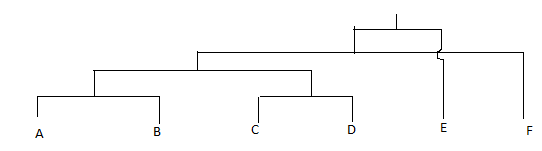
\includegraphics{2a1.png}\\

\part{2}\\
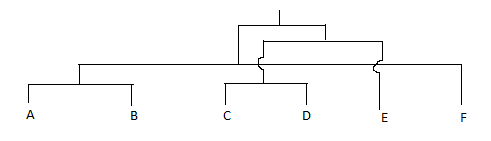
\includegraphics{2a2.png}\\

\part{3}
Swap the distances for AD and BF. 

\question{2.b}{Clustering: Which clustering method should we use?}
\part{1}
This looks like heirarchical clustering with single link. Points close to each other are clustered together, and since the clusters are long and skinny, they are more likely to be single link. 

\part{2}
This looks like K-means custering. Points are clustered in a circular pattern, and k-means attempts to minimize the distance between the points and the cluster centroids.

\part{3}
This looks like GMM. Because the two clusters seem to cross each other but still have a distinct shape, it seems like they follow a two-dimensional probability distribution, as is the case in GMM. 

\question{3.a}{Semi-Supervised Learning}
\part{1}
To show that $d(h_1, h_2)$ is a distance metric, we must show that it is symmetric, non-negative and satisfies the triangle inequality.

Symmetry:\\
\begin{eqnarray*}
d(h_1, h_2) &=& \int |h_1(x) - h_2(x)|p(x)dx\\
d(h_2, h_1) &=& \int |h_2(x) - h_1(x)|p(x)dx\\
&=& \int |-(h_1(x) - h_2(x))|p(x)dx \ by \ a-b = -(b-a) \ factoring\\
&=& \int |h_1(x) - h_2(x)|p(x)dx \ by \ def \ of \ absolute \ value\\
\Rightarrow d(h_2, h_1) &=& d(h_1, h_2)\\
\end{eqnarray*}

and

Assume $h_1 = h_2$.
\begin{eqnarray*}
d(h_1, h_2) &=&  d(h_1, h_1)\\
&=& \int |h_1(x) - h_1(x)|p(x)dx\\
&=& \int 0*p(x)dx\\
&=& 0\\
\Rightarrow h_1 = h_2 &\Rightarrow& d(h_1, h_2) = 0
\end{eqnarray*}

Assume $d(h_1, h_2) = 0$.
\begin{eqnarray*}
\Rightarrow p(x) = 0 \ &or& \ |h_1(x) - h_2(x)| = 0\\
Case \ p(x) &=& 0, \ trivial\\
Case \ |h_1(x) - h_2(x)| &=& 0\\
\Rightarrow h_1(x) - h_2(x) = 0\\
\Rightarrow h_1(x) = h_2(x)\\
\Rightarrow d(h_1, h_2) = 0 &\Rightarrow&  h_1 = h_2\\
\end{eqnarray*}

Together, these two proofs show prove that $h_1 = h_2 \iff d(h_1, h_2) = 0$. 



Non-negative:\\
We know that an integral is essentially a sum of, and so we know that if all the terms of the sum are non-negative, the total sum will also be non-negative. So, we can show that $d(h_1, h_2)$ is non-negative by showing each term is non-negative. In particular, we want to show that $|h_1(x) - h_2(x)|p(x) \geq 0$. By looking at the terms, we know that $p(x)$ is a probability distribution function, and it is impossible for a probability to be negative, and so that term is non-negative. Furthermore, by definition of absolute value, we know that the term $|h_1(x) - h_2(x)|$ must be non-negative. Therefore, we have a product of two non-negative terms, which we know must also be non-negative. So, the entire integral is non-negative. QED.

Triangle Inequality:\\
\begin{eqnarray*}
WTS \ d(h_1, h_2) &=& d(h_1, h_3) + d(h_3, h_2)\\
&=& \int |h_1(x) - h_3(x)|p(x)dx +  \int |h_3(x) - h_2(x)|p(x)dx\\
&=& \int |h_1(x) - h_3(x)|p(x) + |h_3(x) - h_2(x)|p(x)dx\\
&=& \int (|h_1(x) - h_3(x)| + |h_3(x) - h_2(x)|)p(x)dx\\
&=& \int (|h_1(x) - h_3(x) + h_3(x) - h_2(x)|)p(x)dx\\
&=& \int |h_1(x) - h_2(x)|p(x)dx\\
\end{eqnarray*}

So, $d(h_1, h_2)$ is a distance metric because it satisfies all the criteria.

\part{2}
You can estimate $d(h_1, f)$ by using L and U with $h_1$ and seeing how different it is from the true labels (as they would be predicted by $f$). Then, you can estimate $d(h_1, h_2)$ by using the triangle inequality and splitting it into $d(h_1, f) + d(f, h_2)$ and using the first strategy.

\question{3.b}{Semi-Supervised Learning}
\part{1}
I would pick $n=2$ because all the hypotheses after that are overfitting. I wrote a Python script that outputted the squared error for each hypothesis, and got the following values for hypotheses $h_1$ through $h_6$ (respectively): 207, 205, 234661, 821984, 3, 1. Furthermore, I also used this script to calculate additional distance metrics (in particular, $\hat{d}(h_i, f)$), which in this case turned out to be 1 for $i \in \{1, 2, 3, 4, 5, 6\}$. This means that since we have the heuristic of continue training until $\hat{d}(h_i, h_{i-1})$ fails to satisfy the triangle inequality, we should train only until $\hat{d}(h_i, h_{i-1}) \leq \hat{d}(h_i, f) + \hat{d}(h_{i-1}, f)$ no longer holds. This occurs when $i=3$, because $\hat{d}(h_3, h_2) = 3.244 \not \leq 2.0$, and so the triangle inequality no longer holds. Thus, I pick $n=2$.

\question{4}{Programming: K-Means}
\part{1}
Since we have the true labels, we can evaluate the clustering performance by seeing the precision of the run, and so when starting with randomly selected centroids, the "best" results would be the ones with the highest precision. (In the case that we did not have the true labels, the lowest value of the objective function of K-means could have been used. Note that it is possible to have the lowest objective function value but still not the best precision.)

\part{2}
The objective function is monotonically decreasing as the number of iterations increases.\\
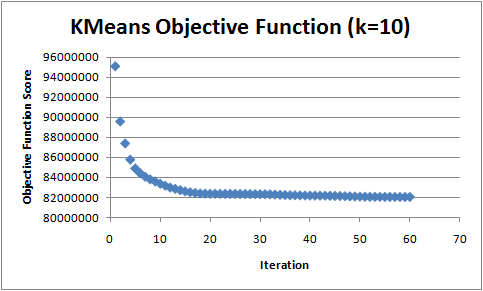
\includegraphics{q4b.png}\\

\part{3}
The algorithm converges much, much earlier (17 iterations instead of ~60) than when $k=10$, and also the overall objective function score asymptotes to a lower value when $k=16$ than when $k=10$.\\
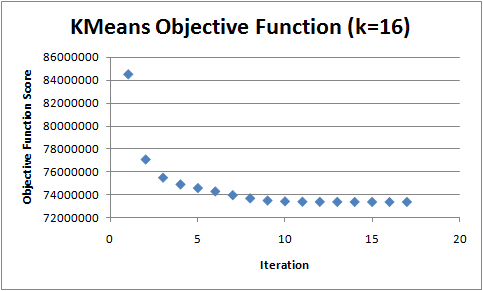
\includegraphics{q4c.png}\\

\part{4}
\begin{table}
    \begin{tabular}{|c|c|c|}
        \hline
        K  & Accuracy & Objective Function Score \\ \hline
        1  & 0.114    & 1276236239               \\ 
        5  & 0.449    & 955013392                \\ 
        10 & 0.6346   & 828455714                \\ 
        16 & 0.6882   & 732872757                \\ 
        20 & 0.733    & 695375664                \\
        \hline
    \end{tabular}
\end{table}

\part{5}
By looking at the true labels, it seems like there were only 10 clusters (as there were only 10 labels, 0-9). The labels of the clusters when $k=10$ were relatively evenly distributed (0-9, with the exception of label 5 being replaced with 7). At higher $k$ values, there were many more duplicates that were not evenly distributed, meaning it seemed that the data was overfit and it was splitting an existing large cluster into smaller clusters to account for the larger value of $k$. So, it seems like 10 clusters would be the optimal number, providing that good starting points were chosen. However, because of the way we actually label the clusters after clustering (using the highest count true label to label the entire cluster), we get better accuracy as the number of clusters increase (most likely due to overfitting on the training data - which we want to avoid). Also, it is logical to assume that the final objective function score will decrease as the number of clusters increase because, with more centroids, in general, the distance between a point and it's corresponding cluster's centroid will decrease. This means that the overall objective function will also decrease. 


\end{document}
